\documentclass[a4paper,man,natbib]{apa6}

\usepackage[english]{babel}
\usepackage[utf8x]{inputenc}
\usepackage{amsmath}
\usepackage{graphicx}
\usepackage[colorinlistoftodos]{todonotes}

% override apa6 first paragraph index
% https://tex.stackexchange.com/questions/155028/indentation-apa6-class-for-2nd-paragraphs-after-title
% \makeatletter
%   \b@level@one@skip=-2.5ex plus -1ex minus -.2ex
%   \b@level@two@skip=-2.5ex plus -1ex minus -.2ex
% \makeatother

\title{Supplemental materials for ``An item response theory analysis of the Matrix Reasoning Item Bank (MaRs-IB)''}
\shorttitle{Supplemental materials for ``IRT analysis of MaRs-IB''}
\author{Samuel Zorowitz$^1$, Gabriele Chierchia$^3$, Sarah-Jayne Blakemore$^3$, Nathaniel D. Daw$^{1,2}$}
\affiliation{$^1$Princeton Neuroscience Institute, Princeton University, USA\\$^2$Department of Psychology, Princeton University, USA\\$^3$Department of Psychology, University of Cambridge, Downing Street, Cambridge, UK}

\setcounter{figure}{0}
\setcounter{table}{0}
\renewcommand{\thetable}{S\arabic{table}}
\renewcommand{\thefigure}{S\arabic{figure}}

\begin{document}
\maketitle

\section*{Speed-accuracy trade-offs in Chierchia et al. (2019)}

To investigate the possibility of speed-accuracy trade-offs in the original MaRs-IB data, we looked at the proportion of correct responses to the easiest items (dimension 1/2 items) as a function of the number of participants having reached that item. In all partitions of these data, we found robust positive correlations between proportion correct and number reached (dimension 1 items: $\rho$ = 0.514, p = 0.050; dimension 2 items: $\rho$ = 0.767, p < 0.001; combined: $\rho$ = 0.695, p < 0.001). This result suggests that the participants that did reach items later in the sequence were able to do by sacrificing accuracy for speed. As such, the item-level performance summary released as part of Chierchia et al. (2019) are likely biased indicators of item functioning.

\begin{table}
    \centering
    \begin{tabular*}{\textwidth}{clcr}
    \toprule
    Model & Description & psis-loco & $\Delta$ psis-loco (se) \\
    \midrule
    7 & TK  & 27741.4 & 635.3 (29.7) \\
    8 & TK  & 26962.1 & 665.6 (32.2) \\
    9 & TK & 26585.5 & 633.1 (33.9) \\
    \bottomrule
    \end{tabular*}
    \caption{\label{tab:2}\normalfont Goodness-of-fit of item response models to MaRs-IB data. LOCO values are presented in deviance scale (i.e. smaller numbers indicate better fit). Abbreviations: PSIS = Pareto-smoothed importance sampling; LOCO = leave-one-cluster-out.}
    \label{table:2}
\end{table}

\begin{table}
\centering
\begin{tabular*}{\textwidth}{ccccccllll}
\toprule
 & & & & & & \multicolumn{4}{c}{Spearman rank correlation} \\
\cmidrule(lr){7-10}
Measure & & Mean (SD) & & IQR & &  NFC-10 & PCF-8a & SNS & MaRs-SF \\
\midrule
NFC-10 & & 25.03 (8.27) & & 20.00 -- 31.00 & & - &  &  & \\
PCF-8a   &  & 22.17 (6.29) & & 18.75 -- 26.25 & & 0.27** &  - &  &  \\
SNS   &  & 29.07 (7.48) & & 25.00 -- 35.00 & & 0.46** &  0.29** &  - &   \\
MaRs-SF & &   8.00 (2.53) & &   6.00 -- 10.00 & & -0.04 &  0.04 &  0.14* &  - \\
\bottomrule
\end{tabular*}
\captionsetup{width=1.\textwidth}
\caption{\normalfont Correlations between performance on the MaRs-IB short forms and self-report measures. Abbreviations: IQR = interquartile range; NFC-10 = need for cognition (10-item) scale; PCF = PROMIS cognitive functioning scale (8a); SNS = subjective numeracy scale. \\ ** p < 0.001,  * p < 0.05 (not corrected for multiple comparisons)}
\end{table}

\begin{figure}
\centering
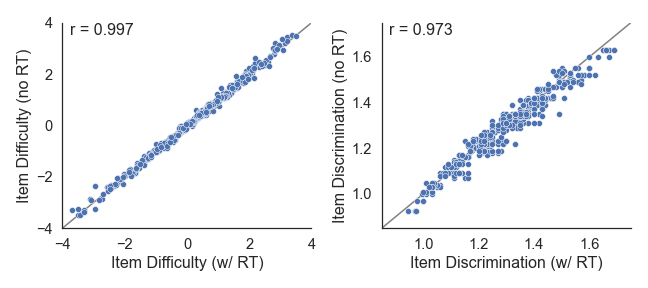
\includegraphics[width=1.0\textwidth]{figures/figS01.png}
\caption{\label{fig:figS01} An example item clone from each of the nine stimulus sets. In each row are three clones of one item template. Though some elementary shapes (e.g. circles, squares) are shared across stimulus sets, the majority of stimuli in each set are unique.}
\end{figure}

\end{document}